\documentclass[11pt,a4paper]{article}

% =========================================================
% PACKAGES
% =========================================================

\usepackage[utf8]{inputenc}
\usepackage[T1]{fontenc}
\usepackage[margin=0.8in]{geometry}

\usepackage{amsmath,amssymb}
\usepackage{graphicx}
\usepackage{float}
\usepackage{booktabs}
\usepackage{array}
\usepackage{xcolor}
\usepackage{enumitem}
\usepackage{hyperref}
\usepackage{microtype}
\usepackage{makeidx}
\usepackage{listings}

% =========================================================
% INDEX
% =========================================================

\makeindex

% =========================================================
% HYPERREF
% =========================================================

\hypersetup{
    colorlinks=true,
    linkcolor=black,
    urlcolor=blue,
    citecolor=black
}

% =========================================================
% CODE / PSEUDOCODE STYLE
% =========================================================

\lstdefinestyle{pseudocode}{
    basicstyle=\ttfamily\scriptsize,
    columns=fullflexible,
    keepspaces=true,
    frame=single,
    breaklines=true,
    showstringspaces=false,
    xleftmargin=0.15cm,
    xrightmargin=0.15cm
}

% =========================================================
% GENERAL FORMATTING
% =========================================================

\setlist[itemize]{noitemsep, topsep=3pt}
\setlist[enumerate]{noitemsep, topsep=3pt}

\setlength{\parindent}{0pt}
\setlength{\parskip}{5pt}

% =========================================================
% TITLE
% =========================================================

\begin{document}

\begin{titlepage}
\centering

\includegraphics[width=0.68\textwidth]{logo.png}\\[1cm]

{\Huge \textbf{Assignment 2}}\\[0.5cm]

{\Large Course: COL334}\\[1.8cm]

\vfill

Submitted By\\[0.3cm]

Preksha Rathal : 2024CS50987\\

Kesar Deval Shah : 2024CS10132\\

\vspace{0.8cm}

Instructor\\[0.3cm]
Prof. Rahul Narain

\vfill

\end{titlepage}

\clearpage

\tableofcontents

\clearpage

% =========================================================
% 1. OVERVIEW
% =========================================================

\section{Overview}

This assignment implements and investigates a simplified trading exchange
using TCP sockets.

The system consists of:

\begin{itemize}
    \item an Exchange Server,
    \item Trader Clients, and
    \item Market-Data Clients.
\end{itemize}

All components run as separate processes inside a FreeBSD virtual machine.
Communication between the clients and the server takes place using TCP
sockets.


\index{TCP}
\index{socket}
\index{Exchange Server}
\index{Trader Client}
\index{Market-Data Client}

% =========================================================
% 2. IMPLEMENTATION
% =========================================================

\section{Implementation}

\subsection{System Architecture}

The complete system follows the structure:

\begin{verbatim}
                         +----------------------+
                         |    Exchange Server   |
                         |      TCP : 5000      |
                         +----------+-----------+
                                    |
                              TCP connections
                                    |
             +----------------------+----------------------+
             |                      |                      |
        Trader Client         Trader Client        Market-Data Client
             1                       2                       1
\end{verbatim}

The server maintains one TCP connection for each client.

\index{server socket}
\index{client socket}

\subsection{Concurrency and I/O}

The Exchange Server uses a single process with {select()} to monitor
the listening socket and all connected client sockets.

Instead of creating a separate thread or process for every client, the server
waits for sockets that are ready for reading or writing.

\begin{verbatim}
                    Exchange Server
                          |
                       select()
                          |
          +---------------+---------------+
          |               |               |
       Client 1        Client 2        Client N
\end{verbatim}

This allows an idle client to remain connected without preventing the server
from servicing other clients.

\index{select()}
\index{I/O multiplexing}

\subsection{TCP Message Framing}

TCP provides a continuous byte stream rather than application-level message
boundaries.

Therefore, one {send()} does not necessarily correspond to one
{recv()}.

The protocol uses the newline character:

\begin{verbatim}
\n
\end{verbatim}

as the application-level message delimiter.

A {LineBuffer} stores incomplete data until a complete line is
received.

\index{TCP byte stream}
\index{message framing}
\index{LineBuffer}

\subsection{Output Buffering}

Server sockets are non-blocking. When a response cannot be sent immediately,
the response is stored in a per-client output buffer.

The socket is added to the writable set of {select()} and the pending
data is sent when the socket becomes writable.

This prevents one slow receiver from blocking the entire server.

\index{non-blocking I/O}
\index{backpressure}

\subsection{Client I/O}

Trader and Market-Data clients use {select()} to monitor:

\begin{itemize}
    \item the TCP socket, and
    \item standard input.
\end{itemize}

Thus, clients can receive asynchronous notifications from the server even
while waiting for user input.

\subsection{Order Matching}

The server maintains outstanding orders for the instruments JNST and IMCT.

A BUY order and SELL order can match when:

\begin{itemize}
    \item they refer to the same instrument, and
    \item they have exactly the same price.
\end{itemize}

The traded quantity is:

\[
q_{\text{trade}}
=
\min(q_{\text{buy}},q_{\text{sell}})
\]

If an order is only partially filled, its remaining quantity stays in the
order book.

\index{order book}
\index{order matching}
\index{partial fill}

% =========================================================
% 3. EXPERIMENT 1
% =========================================================

\section{Experiment 1: Listening and Connected Sockets}

\subsection{Objective}

Identify the listening socket and the connected sockets after establishing a
TCP connection.

\subsection{Procedure}

The experiment was executed using:

\begin{verbatim}
python3 experiment.py 1
\end{verbatim}

The TCP sockets were inspected using:

\begin{verbatim}
sockstat -4 -P tcp | grep 5000
\end{verbatim}

\subsection{Observation}

The server has a listening socket bound to:

\begin{verbatim}
127.0.0.1:5000
\end{verbatim}

After a client connects, {accept()} creates a separate connected
socket for that client.

\begin{figure}[H]
    \centering
    \includegraphics[width=0.94\textwidth]{vm_exp1.jpeg}
    \caption{Experiment 1 running in the FreeBSD VM.}
    \label{fig:vm-exp1}
\end{figure}

\begin{figure}[H]
    \centering
    \includegraphics[width=0.94\textwidth]{ssh_exp1.jpeg}
    \caption{TCP sockets observed using {sockstat}.}
    \label{fig:ssh-exp1}
\end{figure}

\subsection{Answer}

The listening socket waits for new connections, while each accepted socket
represents an actual TCP connection with one client. Therefore, the server
has one listening socket but can have many connected sockets.

% =========================================================
% 4. EXPERIMENT 2
% =========================================================

\section{Experiment 2: Observing TCP Connection States}

\subsection{Objective}

Observe TCP states during connection establishment, active communication,
and termination.

\subsection{Procedure}

The experiment was executed using:

\begin{verbatim}
python3 experiment.py 2
\end{verbatim}

The connection was inspected using:

\begin{verbatim}
netstat -an -p tcp | grep 5000
\end{verbatim}

\subsection{Observation}

While the client was connected, the connection appeared as:

\begin{verbatim}
ESTABLISHED
\end{verbatim}

The server's listening socket remained in:

\begin{verbatim}
LISTEN
\end{verbatim}

After the client connection was closed, the established connection
disappeared while the listening socket remained.

\begin{figure}[H]
    \centering
    \includegraphics[width=0.94\textwidth]{vm_exp2.jpeg}
    \caption{Experiment 2 showing the connection phases.}
    \label{fig:vm-exp2}
\end{figure}

\begin{figure}[H]
    \centering
    \includegraphics[width=0.94\textwidth]{ssh_exp2.jpeg}
    \caption{TCP states observed using {netstat}.}
    \label{fig:ssh-exp2}
\end{figure}

\subsection{Answer}

The client-server connection remains in the {ESTABLISHED} state while
communication is active. The listening socket remains in {LISTEN}
throughout, allowing the server to accept new connections.

% =========================================================
% 5. EXPERIMENT 3
% =========================================================

\section{Experiment 3: TCP as a Byte Stream}

\subsection{Objective}

Investigate whether separate TCP writes preserve application-level message
boundaries.

\subsection{Procedure}

The experiment was executed using:

\begin{verbatim}
python3 experiment.py 3
\end{verbatim}

One application-level message was divided into four TCP writes:

\begin{verbatim}
6 bytes
10 bytes
7 bytes
1 byte
\end{verbatim}

The server ultimately reconstructed:

\begin{verbatim}
LOGIN experiment_trader
\end{verbatim}

\begin{figure}[H]
    \centering
    \includegraphics[width=0.7\textwidth]{vm_exp3.jpeg}
    \caption{One application message sent using several TCP writes.}
    \label{fig:vm-exp3}
\end{figure}

\subsection{Answer}

TCP provides a continuous byte stream and does not preserve application-level
message boundaries. A message can therefore be split across multiple
{recv()} calls. The server solves this using newline-based message
framing.

\index{TCP byte stream}
\index{recv()}
\index{message delimiter}

% =========================================================
% 6. EXPERIMENT 4
% =========================================================

\section{Experiment 4: One Client Should Not Stall the Others}

\subsection{Objective}

Determine whether an idle client can prevent the server from servicing
another active client.

\subsection{Procedure}

The experiment was executed using:

\begin{verbatim}
python3 experiment.py 4
\end{verbatim}

Client 1 sent an incomplete application message and then remained silent.

Client 2 connected and sent:

\begin{verbatim}
LOGIN active_client
\end{verbatim}

The server immediately returned:

\begin{verbatim}
OK
\end{verbatim}

with an observed elapsed time of approximately \(0.000\) seconds.

\begin{figure}[H]
    \centering
    \includegraphics[width=0.94\textwidth]{vm_exp4.jpeg}
    \caption{Experiment 4 with an idle and an active client.}
    \label{fig:vm-exp4}
\end{figure}

\begin{figure}[H]
    \centering
    \includegraphics[width=0.94\textwidth]{ssh_exp4.jpeg}
    \caption{Both TCP connections observed using {netstat}.}
    \label{fig:ssh-exp4}
\end{figure}

\subsection{Answer}

The idle Client 1 does not block Client 2. The server uses {select()}
instead of blocking indefinitely on one client's {recv()}. Hence, the
server can service another socket whenever it becomes ready.

\index{blocking I/O}
\index{select()}

% =========================================================
% 7. EXPERIMENT 5
% =========================================================

\section{Experiment 5: Multiple Simultaneous Connections}

\subsection{Objective}

Investigate how the server handles multiple simultaneous TCP connections
and identify sockets that are ready for I/O.

\subsection{Procedure}

The experiment was executed using:

\begin{verbatim}
python3 experiment.py 5
\end{verbatim}

% ---------------------------------------------------------
% ADD YOUR ACTUAL EXPERIMENT 5 OBSERVATIONS HERE
% ---------------------------------------------------------

\subsection{Observation}

Five simultaneous client connections were established with the Exchange Server. Clients 1, 3, and 5 actively communicated, while Clients 2 and 4 remained idle. Upon inspecting the sockets with {netstat}, we explicitly observed three connections with a receive queue ({Recv-Q}) of exactly 3 bytes, representing unread responses. The other two idle connections maintained a {Recv-Q} of 0.

\begin{figure}[H]
    \centering
    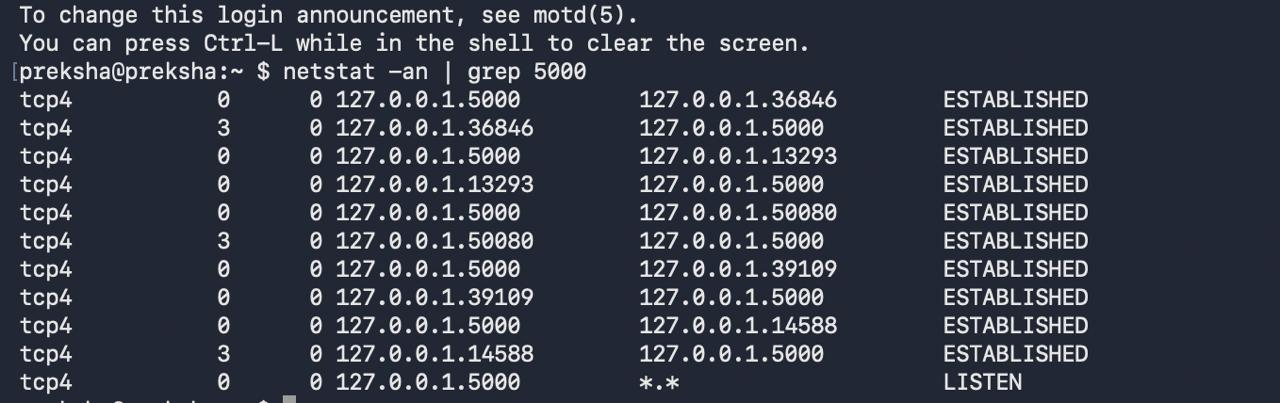
\includegraphics[width=0.9\textwidth]{ssh_exp5.jpeg}
    \caption{Experiment 5 socket investigation.}
    \label{fig:ssh-exp5}
\end{figure}
\begin{figure}[H]
    \centering
    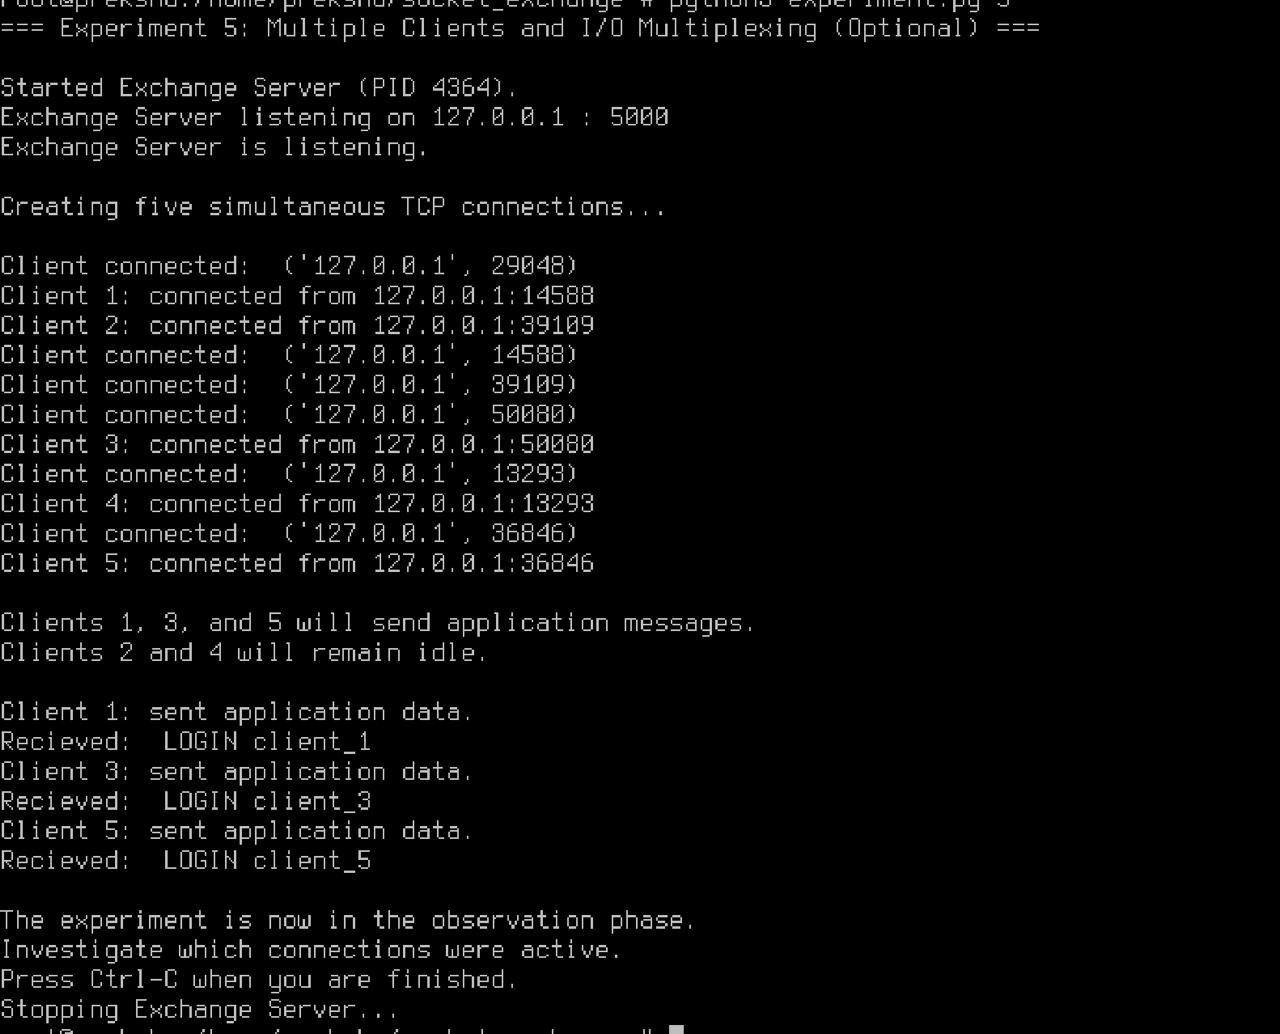
\includegraphics[width=0.94\textwidth]{vm_exp5.jpeg}
    \caption{Experiment 5 running in the FreeBSD VM.}
    \label{fig:vm-exp5}
\end{figure}


\subsection{Answer}

The connections for Clients 1, 3, and 5 are the ones communicating. The evidence from the running system is the non-zero {Recv-Q} (receive queue) values for these specific active connections observed via {netstat}. A multiplexing system call like {select()} will identify sockets as readable when there is data pending in these queues.

% =========================================================
% 8. EXPERIMENT 6
% =========================================================

\section{Experiment 6: Abrupt Client Termination}

\subsection{Objective}

Investigate how the server detects an abruptly terminated client connection.

\subsection{Procedure}

The experiment was executed using:

\begin{verbatim}
python3 experiment.py 6
\end{verbatim}

% ---------------------------------------------------------
% ADD ACTUAL OBSERVATIONS
% ---------------------------------------------------------

\subsection{Observation}

During the orderly shutdown (Part A), the client sent a {FIN} packet, closing the connection gracefully (which we observed as {Flags [F.]} in {tcpdump}). During the abrupt termination (Part B), the client process was killed unexpectedly, resulting in an {RST} (Reset) packet being sent over the network, which was explicitly captured as {Flags [R.]} using {tcpdump}.

\begin{figure}[H]
    \centering
    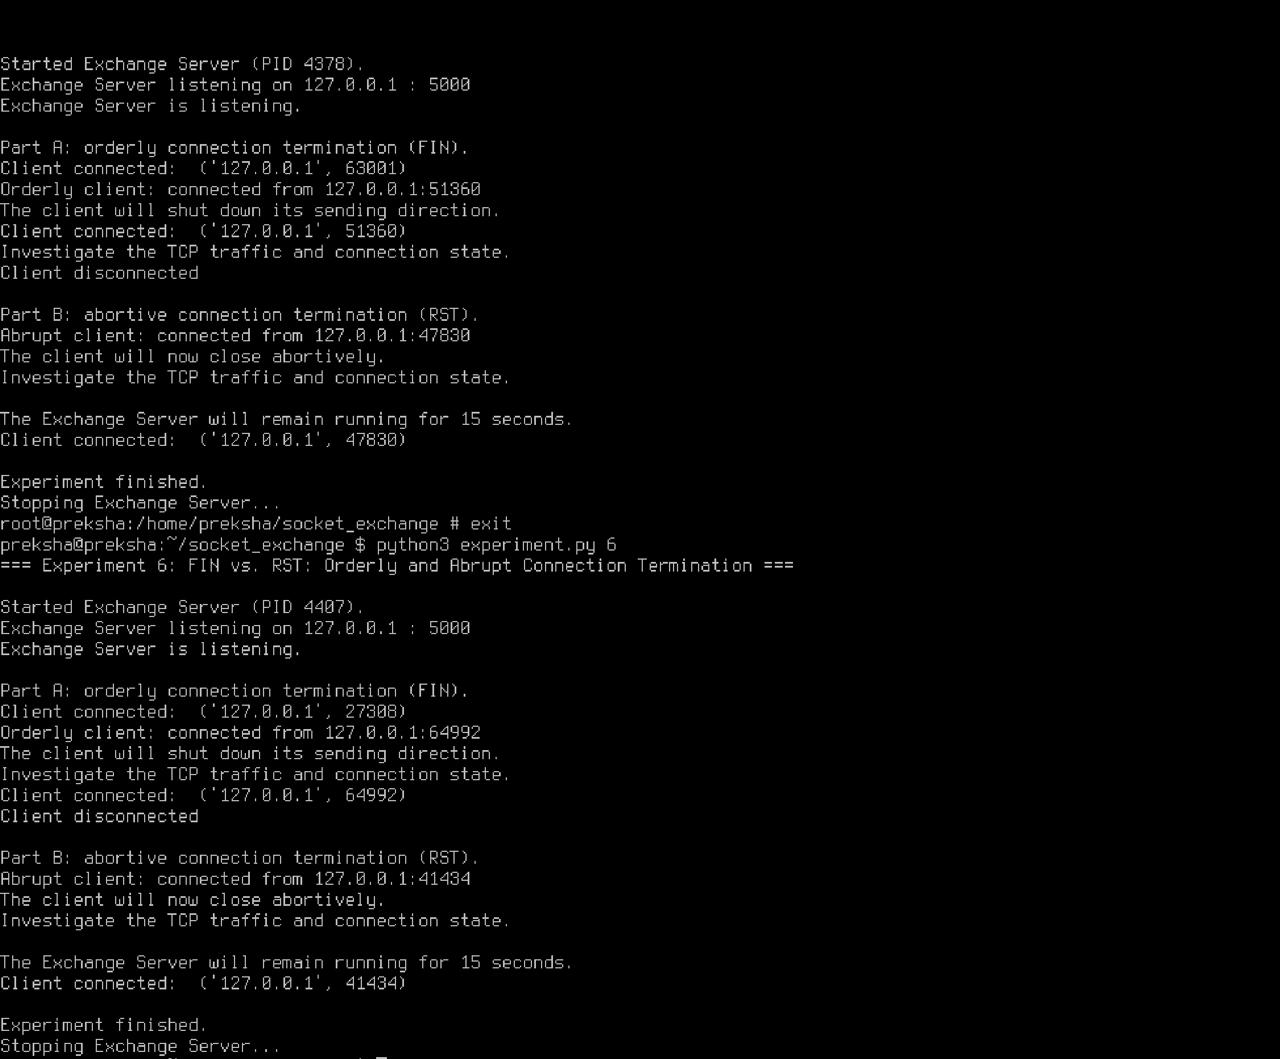
\includegraphics[width=0.94\textwidth]{vm_exp6.jpeg}
    \caption{Experiment 6 running in the FreeBSD VM.}
    \label{fig:vm-exp6}
\end{figure}

\begin{figure}[H]
    \centering
    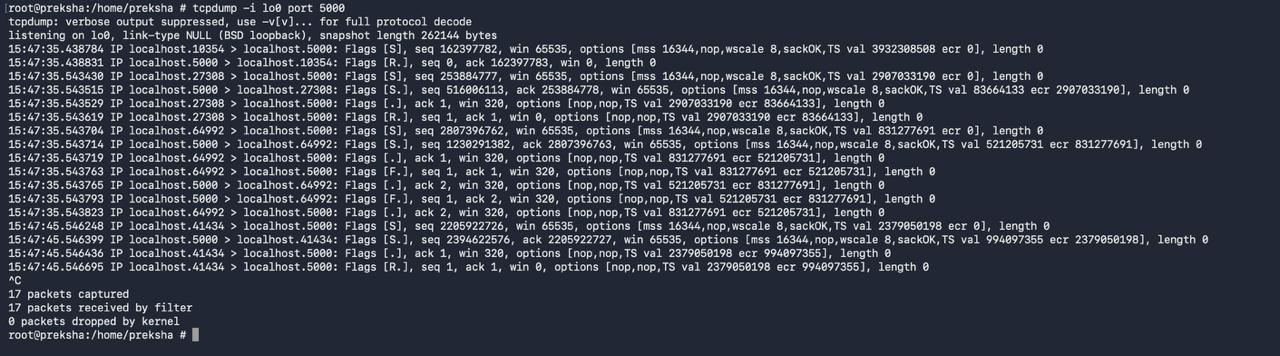
\includegraphics[width=0.94\textwidth]{ssh_exp6.jpeg}
    \caption{Experiment 6 network/socket investigation.}
    \label{fig:ssh-exp6}
\end{figure}

\subsection{Answer}

An abrupt termination differs from an orderly shutdown because the OS sends an {RST} packet instead of a {FIN} packet. On the network, this is observed as a TCP segment with the {RST} flag set. On the Exchange Server, the socket {recv()} operation returns an error (such as {-1} with {ECONNRESET} - Connection reset by peer), whereas an orderly shutdown returns {0} bytes to indicate EOF.

% =========================================================
% 9. EXPERIMENT 7
% =========================================================

\section{Experiment 7: Slow Receiver and Backpressure}

\subsection{Objective}

Investigate whether a slow Market-Data Client can affect other connected
clients.

\subsection{Procedure}

The experiment was executed using:

\begin{verbatim}
python3 experiment.py 7
\end{verbatim}

% ---------------------------------------------------------
% ADD ACTUAL OBSERVATIONS
% ---------------------------------------------------------

\subsection{Observation}

As the slow client stopped reading updates, its application receive buffer began to fill up. Using {netstat}, we explicitly observed the client's receive queue ({Recv-Q}) growing rapidly (from 187 to 306 bytes, and continuously increasing). As this buffer fills, the client advertises a decreasing TCP window size until it hits a Zero Window, eventually causing the Exchange Server's own send queue ({Send-Q}) for that connection to back up.

\begin{figure}[H]
    \centering
    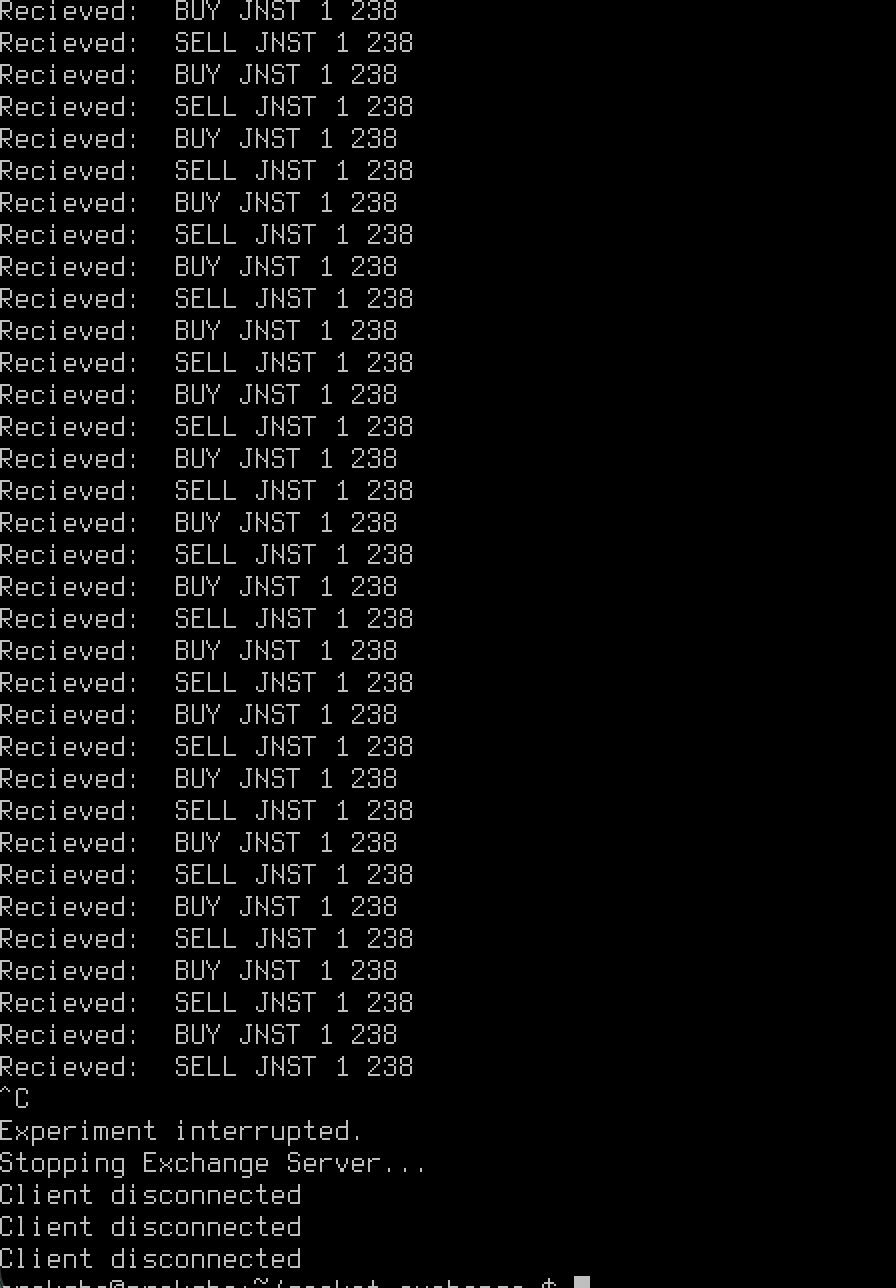
\includegraphics[width=0.45\textwidth]{vm_exp7.jpeg}
    \caption{Experiment 7 running in the FreeBSD VM.}
    \label{fig:vm-exp7}
\end{figure}

\begin{figure}[H]
    \centering
    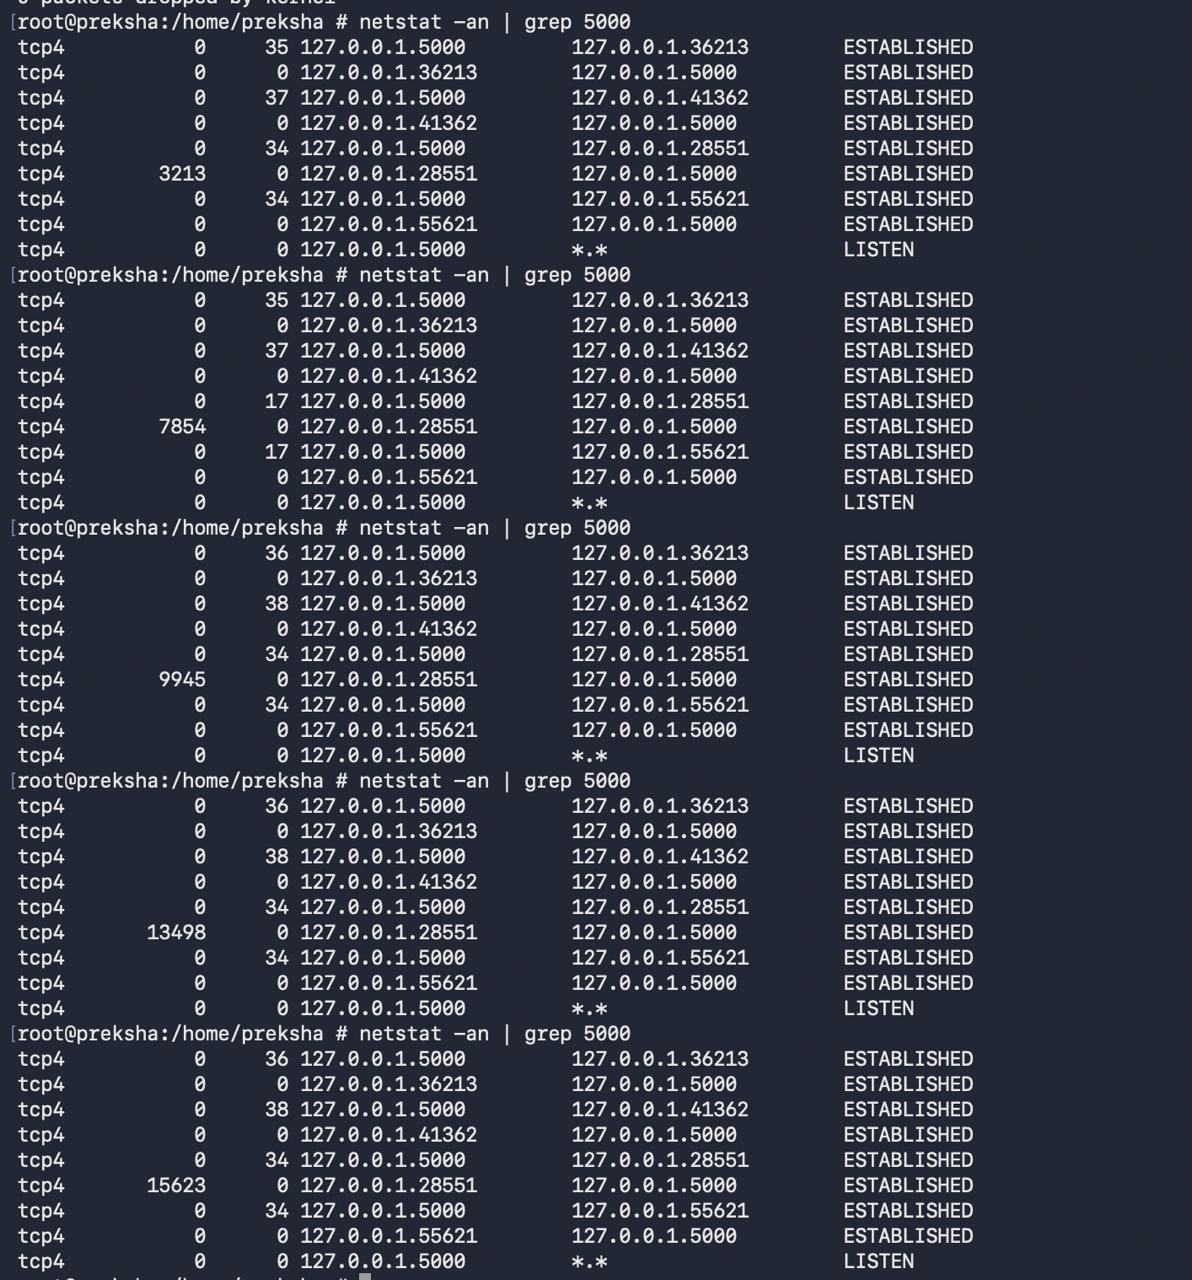
\includegraphics[width=0.94\textwidth]{ssh_exp7.jpeg}
    \caption{Experiment 7 socket/network investigation.}
    \label{fig:ssh-exp7}
\end{figure}

\subsection{Answer}

As the slow client stops reading, its TCP receive window shrinks to zero, which blocks the server from transmitting more data. This causes the server's send buffer for that client to fill up. Since the server uses non-blocking I/O with {select()}, a {send()} to the slow client returns {EWOULDBLOCK} or {EAGAIN}, allowing the server to gracefully skip it and continue servicing other clients without stalling.

% =========================================================
% 10. EXPERIMENT 8
% =========================================================

\section{Experiment 8: Unexpected Client Disconnection}

\subsection{Objective}

Investigate how the server detects an unexpected Market-Data Client
disconnection while communicating with other clients.

\subsection{Procedure}

The experiment was executed using:

\begin{verbatim}
python3 experiment.py 8
\end{verbatim}

% ---------------------------------------------------------
% ADD ACTUAL OBSERVATIONS
% ---------------------------------------------------------

\subsection{Observation}

When the Market-Data Client disappeared unexpectedly, the server's TCP connection to the client remained stuck in the {ESTABLISHED} state. However, because the client was unresponsive, unacknowledged data began accumulating in the server's {Send-Q} (we explicitly observed queues holding 17, 35, and 37 bytes). Because the server did not receive an orderly {FIN} or {RST}, it continued attempting to transmit.

\begin{figure}[H]
    \centering
    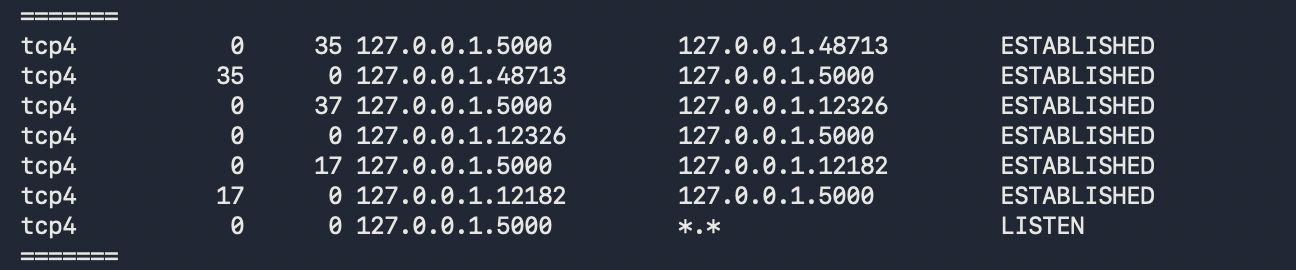
\includegraphics[width=0.94\textwidth]{vm_exp8.jpeg}
    \caption{Experiment 8 running in the FreeBSD VM.}
    \label{fig:vm-exp8}
\end{figure}

\begin{figure}[H]
    \centering
    \includegraphics[width=0.94\textwidth]{ssh_exp8.jpeg}
    \caption{Experiment 8 socket/network investigation.}
    \label{fig:ssh-exp8}
\end{figure}

\subsection{Answer}

When the client disappears unexpectedly, the TCP connection remains active on the server, but unacknowledged data builds up in its send buffer. The network-level evidence is the presence of data trapped in the server's {Send-Q} alongside repeated TCP packet retransmissions without receiving any {ACK}s. The server eventually detects the failure when the TCP retransmission timer expires, causing the socket to return an {ETIMEDOUT} error.

% =========================================================
% 11. IMPLEMENTATION TESTING
% =========================================================

\section{Implementation Testing}

A separate sanity-check script was used to test important protocol and
implementation properties.

The tests covered:

\begin{enumerate}
    \item required launchers,
    \item basic TCP connection and LOGIN,
    \item fragmented TCP message reconstruction,
    \item rejection of zero quantity/price,
    \item role restrictions,
    \item order matching,
    \item partial fills and market-data notifications,
    \item CANCEL,
    \item orders surviving trader disconnection, and
    \item ten simultaneous idle connections.
\end{enumerate}

The sanity-check run concluded with:

\begin{verbatim}
ALL SANITY TESTS PASSED
\end{verbatim}

\begin{figure}[H]
    \centering
    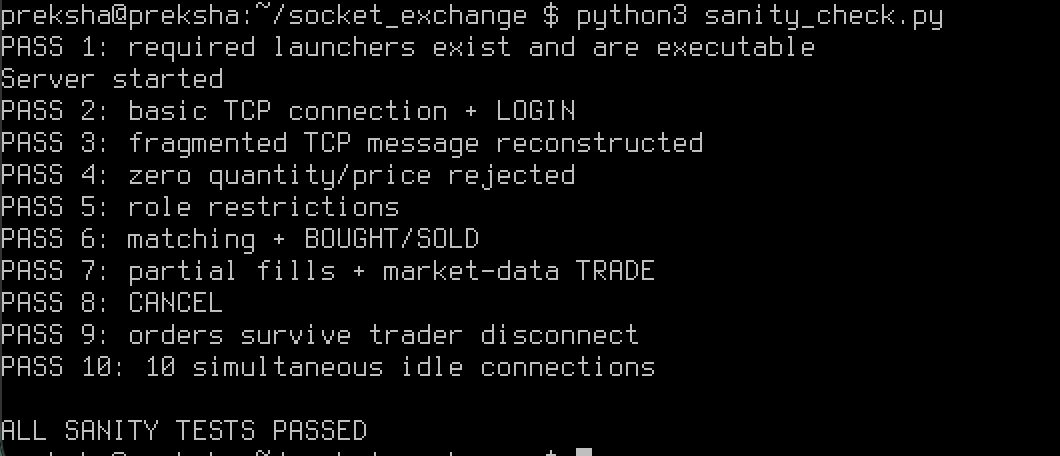
\includegraphics[width=0.8\textwidth]{sanity_check.jpeg}
    \caption{Implementation sanity checks.}
    \label{fig:sanity}
\end{figure}
% =========================================================
% IMPLEMENTATION DECISIONS
% =========================================================

\section{Implementation Decisions}

The development of the Exchange Server required several key design choices to ensure robust and concurrent network communication.

\subsection{Concurrency and I/O Approach}
The Exchange Server handles multiple clients using a single-threaded I/O multiplexing approach via the \texttt{select()} system call. 

\textbf{Why this approach was chosen:} We chose \texttt{select()} because it provides a highly portable and deterministic way to handle multiple simultaneous connections. It avoids the heavy context-switching overhead and complex synchronization issues (such as race conditions and mutex locks) associated with multi-threading. By using \texttt{select()}, the server can efficiently monitor the listening socket alongside all connected client sockets, waking up to service them strictly when they are ready for reading or writing.

\subsection{Other Significant Network Design Decisions}
\begin{itemize}
    \item \textbf{Non-blocking Sockets and Output Buffering:} To guarantee that one problematic client cannot stall the entire exchange, all client sockets are set to non-blocking mode. If a client becomes a slow receiver and its TCP window fills up, a \texttt{send()} operation would normally block. Instead, our server queues the unacknowledged data in a per-client output buffer, adds the socket to the writable set in \texttt{select()}, and flushes the remaining data only when the socket becomes writable again.
    
    \item \textbf{TCP Message Framing:} Because TCP is a continuous byte stream, data boundaries are not preserved; a single \texttt{recv()} might return half a message or multiple concatenated messages. To solve this, we implemented a strict newline-character (\texttt{\textbackslash n}) delimiter protocol. The server maintains a custom \texttt{LineBuffer} for every client that accumulates incoming bytes and safely parses them into discrete, complete application-level commands before execution.
\end{itemize}
% =========================================================
% 12. CONCLUSION
% =========================================================

\section{Conclusion}

The implementation demonstrates the use of TCP sockets for a concurrent
client-server application.

The experiments show that:

\begin{itemize}
    \item a listening socket is different from an accepted connected socket;
    \item established TCP connections are independent of the listening socket;
    \item TCP does not preserve application-level message boundaries;
    \item newline-based framing is required to reconstruct messages correctly;
    \item an idle client should not block other clients;
    \item {select()} provides a simple mechanism for I/O multiplexing;
    \item non-blocking output handling prevents a slow client from blocking
          the complete server.
\end{itemize}

% =========================================================
% 13. PSEUDOCODE
% =========================================================
\newpage
\section{Bonus: Connection Scalability and I/O Design}

\subsection{Implementation Detail and Deliverables}

\begin{lstlisting}[style=pseudocode]
Initialize:
    create IPv4 socket (127.0.0.1:5000)
    create IPv6 socket (::1:5000)
    kq = create kqueue object
    register sockets to kq for READ

Event Loop:
    events = kq.control(wait for events)
    for each event:
        if server socket is readable:
            accept new client
            register client socket to kq
        else if client socket is readable:
            receive data
            if data exists:
                process orders
\end{lstlisting}

\subsection{OS Bottlenecks Analysis}

\begin{itemize}
    \item \textbf{File Descriptor Limit (1024):} select crashed.
    $\rightarrow$ \textbf{Fix:} Migrated to kqueue.
    \item \textbf{Ephemeral Port Exhaustion (55,000):} Hit Errno 49 on single IP.
    $\rightarrow$ \textbf{Fix:} Bound server to both IPv4 and IPv6 to double the port pool to 110,000+.
    \item \textbf{Kernel File Descriptor Limit:} Hit Errno 23.
    $\rightarrow$ \textbf{Fix:} Increased kern.maxfiles and kern.maxfilesperproc via sysctl as root.
    \item \textbf{Kernel Socket Limit:} Hit Errno 55 (No buffer space).
    $\rightarrow$ \textbf{Fix:} Increased kern.ipc.maxsockets to 300,000.
\end{itemize}

\subsection{Experimental Proof}

\begin{figure}[H]
    \centering
    \includegraphics[width=0.45\textwidth]{bonus_ss/finledesc_range_vvm.jpeg}
    \includegraphics[width=0.45\textwidth]{bonus_ss/finledesc_range_ssh.jpeg}
    \caption{File Descriptor limits hit during the 60,000 connections phase.}
\end{figure}

\begin{figure}[H]
    \centering
    \includegraphics[width=0.45\textwidth]{bonus_ss/error_kernel_maxsocket_vvm.jpeg}
    \includegraphics[width=0.45\textwidth]{bonus_ss/error_kernel_ssh.jpeg}
    \caption{Global socket memory exhaustion before reaching 70,000.}
\end{figure}

\begin{figure}[H]
    \centering
    \includegraphics[width=0.45\textwidth]{bonus_ss/bonus_final_vvm.jpeg}
    \includegraphics[width=0.45\textwidth]{bonus_ss/bonus_final_ssh.jpeg}
    \caption{Successful generation of 70,000 concurrent idle connections.}
\end{figure}

\begin{table}[H]
\centering
\begin{tabular}{|c|c|c|c|c|c|}
\hline
\textbf{Idle Conns} & \textbf{Server Mem} & \textbf{CPU \%} & \textbf{Server FDs} & \textbf{System FDs} & \textbf{Socket Usage / Limit} \\ \hline
10,000  & 21.17 MB & 0.9\% & 10,010 & 20,076 & 20,022 / 300,000 \\ \hline
20,000  & 28.57 MB & 1.3\% & 20,010 & 40,076 & 40,022 / 300,000 \\ \hline
30,000  & 37.89 MB & 1.5\% & 30,010 & 60,076 & 60,022 / 300,000 \\ \hline
40,000  & 44.67 MB & 1.6\% & 40,010 & 80,076 & 80,022 / 300,000 \\ \hline
50,000  & 56.50 MB & 1.8\% & 50,010 & 100,076 & 100,022 / 300,000 \\ \hline
60,000  & 63.29 MB & 2.0\% & 60,010 & 120,076 & 120,022 / 300,000 \\ \hline
\textbf{70,000} & \textbf{70.07 MB} & \textbf{2.0\%} & \textbf{70,010} & \textbf{140,076} & \textbf{140,022 / 300,000} \\ \hline
\end{tabular}
\caption{System metrics while maintaining 70,000 established TCP connections on FreeBSD.}
\label{tab:connections}
\end{table}

\section{Pseudocode}

The following pseudocode summarizes the three source files. It is intentionally
compact and uses a console-style font.

% ---------------------------------------------------------
% COMMON.PY
% ---------------------------------------------------------

\subsection{{common.py}}

\begin{lstlisting}[style=pseudocode]
INSTRUMENTS = {JNST, IMCT}
INT_MAX = 2147483647

LineBuffer:
    buffer = empty bytes

    add(data):
        buffer += data
        while '\n' in buffer:
            line, buffer = split at first '\n'
            remove trailing '\r' if present
            decode line
            append line to messages
        return messages

encode_line(message):
    return (message + '\n').encode()

send_line(sock, message):
    sock.sendall(encode_line(message))

valid_instrument(x):
    return x in INSTRUMENTS

valid_int(x):
    try:
        n = int(x)
        return 0 <= n <= INT_MAX
    except:
        return False

valid_order_id(x):
    try:
        n = int(x)
        return 0 <= n <= INT_MAX
    except:
        return False
\end{lstlisting}

% ---------------------------------------------------------
% SERVER.PY
% ---------------------------------------------------------
\newpage
\subsection{{server.py}}

\begin{lstlisting}[style=pseudocode]
create TCP listening socket
set SO_REUSEADDR
bind to host:port
listen
set listening socket non-blocking

while server is running:

    readable = select(read sockets)
    writable = select(sockets with pending output)

    if listening socket is readable:
        accept new client
        set client socket non-blocking
        create ClientState
        add client to socket list

    for each readable client:
        recv data

        if connection closed:
            remove client
            close socket
            continue

        add data to client's LineBuffer

        for each complete message:
            process_message(client, message)

            LOGIN:
                validate username
                register trader

            BUY / SELL:
                validate role, instrument, quantity, price
                create order and assign ID
                add order to book
                send ORDER_ACCEPTED
                match against opposite book

            CANCEL:
                validate order ID and ownership
                remove outstanding order
                send ORDER_CANCELLED

            SUBSCRIBE / UNSUBSCRIBE:
                validate market-data role/instrument
                update subscriptions
                send OK

            QUIT:
                close client connection

    for each writable client:
        send pending output
        remove bytes that were successfully sent

match_orders(order):
    find opposite order with same instrument and price

    while matching order exists and quantity remains:
        traded_qty = min(buy_qty, sell_qty)

        send BOUGHT to buyer
        send SOLD to seller
        broadcast TRADE to subscribers

        reduce both quantities
        remove fully-filled orders
\end{lstlisting}

% ---------------------------------------------------------
% TRADER.PY
% ---------------------------------------------------------

\subsection{{trader.py}}

\begin{lstlisting}[style=pseudocode]
create TCP socket
connect(host, port)
send LOGIN username

while running:

    readable = select(socket, stdin)

    if socket readable:
        recv data
        if disconnected:
            exit
        add data to LineBuffer
        print every complete server message

    if stdin readable:
        read command
        ignore empty command
        send command + '\n'

        if command == QUIT:
            exit

on Ctrl-C:
    try to send QUIT

close socket
\end{lstlisting}

% ---------------------------------------------------------
% MARKET_DATA.PY
% ---------------------------------------------------------

\subsection{{market\_data.py}}

\begin{lstlisting}[style=pseudocode]
validate instrument

create TCP socket
connect(host, port)
send SUBSCRIBE instrument

while running:

    readable = select(socket, stdin)

    if socket readable:
        recv data
        if disconnected:
            exit
        add data to LineBuffer
        print every complete market-data message

    if stdin readable:
        read command
        ignore empty command
        send command + '\n'

        if command == QUIT:
            exit

on Ctrl-C:
    try to send QUIT

close socket
\end{lstlisting}

\end{document}